%!TEX TS-program = xelatex
%!TEX encoding = UTF-8 Unicode

\documentclass[11pt,tikz,border=1]{standalone}
\usepackage[default,mdseries=Light,bfseries=Medium,path=../fonts]{cjkfonts}
\usetikzlibrary{calc,positioning}

% file: westernfonts.tex

\newcommand{\fontdir}[0]{/usr/local/texlive/2015/texmf-dist/fonts/}
\newcommand{\robotodir}[0]{\fontdir/truetype/google/roboto/}
\newcommand{\sourcecodeprodir}[0]{\fontdir/opentype/adobe/sourcecodepro/}
\newcommand{\sourceserifprodir}[0]{\fontdir/opentype/adobe/sourceserifpro/}

\newcommand{\robotomd}[0]{Light}
\newcommand{\robotobf}[0]{Medium}
\newcommand{\robotoit}[0]{LightItalic}
\newcommand{\robotobi}[0]{MediumItalic}
\newcommand{\codepromd}[0]{Light}
\newcommand{\codeprobf}[0]{Medium}
\newcommand{\codeproit}[0]{LightIt}
\newcommand{\codeprobi}[0]{MediumIt}
\newcommand{\serifpromd}[0]{Light}
\newcommand{\serifprobf}[0]{Semibold}

\newfontfamily\Roboto{Roboto}[
  Extension=.ttf,
  Path=\robotodir,
  UprightFont=*-Regular,
  BoldFont=*-Bold,
  ItalicFont=*-RegularItalic,
  BoldItalicFont=*-BoldItalic]

\newfontfamily\SourceCodePro{SourceCodePro}[
  Extension=.otf,
  Path=\sourcecodeprodir,
  UprightFont=*-\codepromd,
  BoldFont=*-\codeprobf,
  ItalicFont=*-\codeproit,
  BoldItalicFont=*-\codeprobi]

\newfontfamily\SourceSerifPro{SourceSerifPro}[
  Extension=.otf,
  Path=\sourceserifprodir,
  UprightFont=*-\serifpromd,
  BoldFont=*-\serifprobf]

\newcommand{\serif}[0]{\SourceSerifPro}

\newfontfamily\RobotoThin{Roboto}[
  Extension=.ttf,
  Path=\robotodir,
  UprightFont=*-Thin,
  ItalicFont=*-ThinItalic]

\newfontfamily\RobotoLight{Roboto}[
  Extension=.ttf,
  Path=\robotodir,
  UprightFont=*-Light,
  ItalicFont=*-LightItalic]

\newfontfamily\RobotoRegular{Roboto}[
  Extension=.ttf,
  Path=\robotodir,
  UprightFont=*-Regular,
  ItalicFont=*-RegularItalic]

\newfontfamily\RobotoMedium{Roboto}[
  Extension=.ttf,
  Path=\robotodir,
  UprightFont=*-Medium,
  ItalicFont=*-MediumItalic]

\newfontfamily\RobotoBold{Roboto}[
  Extension=.ttf,
  Path=\robotodir,
  UprightFont=*-Bold,
  ItalicFont=*-BoldItalic]

\newfontfamily\RobotoBlack{Roboto}[
  Extension=.ttf,
  Path=\robotodir,
  UprightFont=*-Black,
  ItalicFont=*-BlackItalic]

\newcommand{\setdefaultwesternfonts}[0]{
  
  \setmainfont{Roboto}[
    Extension=.ttf,
    Path=\robotodir,
    UprightFont=*-\robotomd,
    BoldFont=*-\robotobf,
    ItalicFont=*-\robotoit,
    BoldItalicFont=*-\robotobi]

  \setsansfont{Roboto}[
    Extension=.ttf,
    Path=\robotodir,
    UprightFont=*-\robotomd,
    BoldFont=*-\robotobf,
    ItalicFont=*-\robotoit,
    BoldItalicFont=*-\robotobi]

  \setmonofont{SourceCodePro}[
    Extension=.otf,
    Path=\sourcecodeprodir,
    UprightFont=*-\codepromd,
    BoldFont=*-\codeprobf,
    ItalicFont=*-\codeproit,
    BoldItalicFont=*-\codeprobi]

}



\begin{document}
  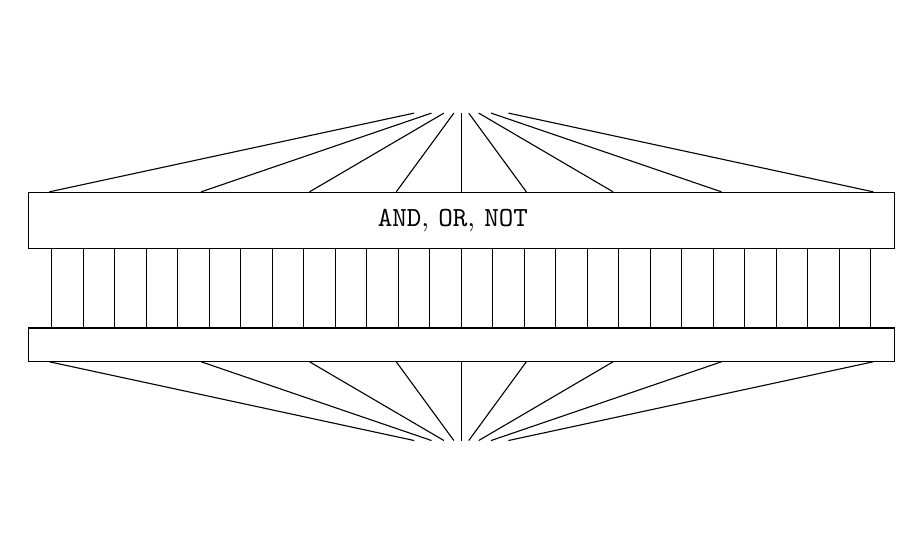
\begin{tikzpicture}[font={\RobotoLight}]

    \foreach \x in {0,...,26}
      \draw (\x * 0.4,0) -- (\x * 0.4, 1);

    \coordinate (layer1bottom) at (5.2,1);
    \coordinate (layer2top) at (5.2,0);
    \node(layer1) [above,rectangle,draw,minimum width=11cm,inner sep=6pt] at (layer1bottom) {
      电路元件(\texttt{AND}, \texttt{OR}, \texttt{NOT} 等)的第一层
    };

    \node(layer2) [below,rectangle,draw,minimum width=11cm,inner sep=6pt] at (layer2top) {
      电路元件的第二层
    };
    
    \node(input) [above=of layer1] {
      \begin{tabular}{c}
        外部输入\\
        (键盘等等)
      \end{tabular}
    };
    
    \node(output) [below=of layer2] {
      \begin{tabular}{c}
        外部输出\\
        (屏幕等等)
      \end{tabular}
    };

    \coordinate (t0) at (layer1.north);
    \coordinate (t1) at (layer1.north east);
    \coordinate (t2) at (layer1.north west);
    \coordinate (i0) at (input.south);
    \coordinate (i1) at (input.south east);
    \coordinate (i2) at (input.south west);
    
    \draw (i0) to (t0);
    \foreach \x in {0.15,0.35,0.6,0.95}
      \draw ($ (i0)!\x!(i1) $) to ($ (t0)!\x!(t1) $);
    \foreach \x in {0.15,0.35,0.6,0.95}
      \draw ($ (i0)!\x!(i2) $) to ($ (t0)!\x!(t2) $);

    \coordinate (b0) at (layer2.south);
    \coordinate (b1) at (layer2.south east);
    \coordinate (b2) at (layer2.south west);
    \coordinate (o0) at (output.north);
    \coordinate (o1) at (output.north east);
    \coordinate (o2) at (output.north west);

    \draw (b0) to (o0);
    \foreach \x in {0.15,0.35,0.6,0.95}
      \draw ($ (b0)!\x!(b1) $) to ($ (o0)!\x!(o1) $);
    \foreach \x in {0.15,0.35,0.6,0.95}
      \draw ($ (b0)!\x!(b2) $) to ($ (o0)!\x!(o2) $);

  \end{tikzpicture} 
\end{document}
